% debut d'un fichier latex standard
\documentclass[a4paper,12pt,oneside]{article}
\usepackage[top=3cm, bottom=3.5cm]{geometry}
% pour l'inclusion de figures en eps,pdf,jpg,....
\usepackage{graphicx}
\usepackage{wrapfig}
\usepackage{subcaption}
\usepackage{siunitx}
% quelques symboles mathematiques en plus
\usepackage{amsmath}
% le tout en langue francaise
\usepackage[french]{babel}
\usepackage[T1]{fontenc}
% on peut ecrire directement les characteres avec l'accent
% a utiliser sur Linux/Windows
\usepackage[utf8]{inputenc}
\usepackage[rightcaption
]{sidecap}
\usepackage[export]{adjustbox}



%Pour du code non interprété
\usepackage{verbatim}
\usepackage{verbdef}% http://ctan.org/pkg/verbdef
% a utiliser sur le Mac
%\usepackage[applemac]{inputenc}
% pour l'inclusion de links dans le document (pdflatex)
\usepackage[colorlinks,bookmarks=false,linkcolor=blue,urlcolor=blue]{hyperref}
%
\usepackage{caption}
\usepackage{float}
% quelques abreviations utiles
\def \be {\begin{equation}}
\def \ee {\end{equation}}
\def \bf {\begin{figure}}
\def \ef {\end{figure}}
\def \dd  {{\rm d}}
\def \t {\theta}
\def \vt {\Dot{\theta}}

\newcommand{\norme}[1]{\left\Vert #1 \right\Vert}
%
\newcommand{\mail}[1]{{\href{mailto:#1}{#1}}}
\newcommand{\ftplink}[1]{{\href{ftp://#1}{#1}}}












%%%%%%%%%%%%%%%%%%%%%%%%%%%%%%%%%%%%%%%%%%%%%%%%%%%%%%%%%%%%%%%%%%%%%%%%%%%%%%%%%%%%%%%%%%%%%%%%%%%%%%%%
%%%%%%%%%%%%%%%%%%%%%%%%%%%%%%%%%% le document commence ici %%%%%%%%%%%%%%%%%%%%%%%%%%%%%%%%%%%%%%%%%%%%
%%%%%%%%%%%%%%%%%%%%%%%%%%%%%%%%%%%%%%%%%%%%%%%%%%%%%%%%%%%%%%%%%%%%%%%%%%%%%%%%%%%%%%%%%%%%%%%%%%%%%%%%
\begin{document}
\pagestyle{empty}

% le titre et l'auteur
\title{Problème de chaleur : exercice 5}
\date{\today}
\author{Timothée Dao, Victor Despland\\{\small \mail{timothee.dao@epfl.ch},\mail{victor.despland@epfl.ch}}}
\maketitle
\thispagestyle{empty} %la première page ne prend pas en compte le style courant
 

\clearpage
\tableofcontents



%%%%%%%%%%%%%%%%%%%%%%%%%%%%%%%%%%%%%%%%%%%%%%%%%%%%%%%%%%%%%%%%%%%%%%%%%%%%%%%%%%%%%%%%%%%%%%%%%%%%%%%%
%%%%%%%%%%%%%%%%%%%%%%%%%%%%%%%%%%%%%%%%%%%%%%%%%%%%%%%%%%%%%%%%%%%%%%%%%%%%%%%%%%%%%%%%%%%%%%%%%%%%%%%%
%%%%%%%%%%%%%%%%%%%%%%%%%%%%%%%%%%%%%%%%%%%%%%%%%%%%%%%%%%%%%%%%%%%%%%%%%%%%%%%%%%%%%%%%%%%%%%%%%%%%%%%%

\newpage 
\setcounter{page}{1}
\pagestyle{plain}

\section{Introduction}

\intextsep=-0.5cm
\begin{wrapfigure}{r}{0.4\textwidth}
    \centering
    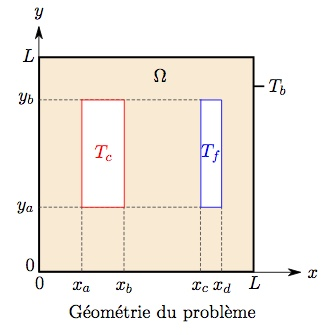
\includegraphics[width=0.5\textwidth]{EX5geom.jpeg}
    \caption{Géométrie du problème \cite{donneeEX5} \label{GeomduP}}
\end{wrapfigure}

Dans ce projet, on étudie le transport de chaleur dans un milieu homogène. On considère une boite carrée de côté $L$ qui possède deux corps rectangulaires à l'intérieur, maintenus respectivement aux températures $T_c$ et $T_f$. Le bord de la boîte est lui à température constante $T_b$. La géométrie est visible sur le schéma de la Fig.\ref{GeomduP}. 
Les données numériques sont sur le tableau Tab.\ref{Tabnum}.

Le flux de chaleur est donné par $\Vec{j}=-\kappa \nabla T$, avec une conductivité thermique constante $\kappa=\SI{1.2}{WK^{-1}m^{-1}}$. De l'équation de continuité $\rho C \frac{\partial T}{\partial t} + \nabla \cdot \Vec{j}=0$, avec une densité de masse $\rho=\SI{1.2}{kg m^{-3}}$ et une capacité thermiques massique $C=\SI{1000}{Jkg^{-1}K^{-1}}$, on peut obtenir l'équation pour le transport de chaleur :
\begin{equation}
    \frac{\partial T}{\partial t}=D\nabla^{2}T
    \label{eq:trans}
\end{equation}
avec $D=\frac{k}{\rho C}$ et $\nabla^{2}T$ le laplacien de température.
\begin{center}

\begin{tabular}{|c|c|c|c|c|c|c|c|c|}
\hline
     $T_b \, \rm[^\circ C]$&  $T_c \, \rm[^\circ C]$& $T_f \, \rm[^\circ C]$&$x_a \, \rm[cm]$ & $x_b \, \rm[cm]$ &$x_c \, \rm[cm]$ &$x_d \, \rm[cm]$ &$y_a \, \rm[cm]$ &$y_b \, \rm[cm]$ \\
     \hline
     $0$&$200$ &$-100$&$2$&$4$&$7.5$&$8.5$&$3$&$8$\\
     \hline
\end{tabular}
 \captionof{table}{Valeurs numériques du problème.}
      \label{Tabnum}
\end{center}

\intextsep=0.5cm



\section{Partie analytique \label{anal}}

On veut montrer analytiquement qu'en régime stationnaire, la somme des puissances émises pas les deux corps est égale à la puissance totale émise par la boîte, c'est-à-dire que $\lim_{t \rightarrow \infty}P_C+P_F=\lim_{t \rightarrow \infty} P_{tot}$.

En tenant compte des termes de densité de source $\pi_f$ et $\pi_c$ provenant des deux corps respectivement froid et chaud, l'équation de continuité s'écrit : $\rho C \frac{\partial T}{\partial t}+ \nabla \cdot \vec{j} = \pi$.
Ce qui donne en régime stationnaire :
\be \nabla \cdot \vec{j} =  \pi_f+\pi_c  \ee
On obtient ainsi finalement, en utilisant le théorème de la divergence et pour le régime stationnaire, 
\be
\begin{array}{r @{{}={}} l}
P_{tot} & \iint_S \vec{j} \, d \vec{s} = \iiint_V \nabla \cdot \vec{j} \, dV = \iiint_V \pi_f + \pi_c \, dV \\ 
        & \iiint_{V_f} \pi_f \, dV +\iiint_{V_c} \pi_c \, dV = \iint_{S_f} \vec{j} \, d \vec{s} + \iint_{S_c} \, \vec{j} d \vec{s} \\ 
        & P_f + P_c
\end{array}
\ee






\section{Méthodes numériques}
\subsection{Discrétisation de la géométrie}
Pour approximer le problème de transport de chaleur, on a besoin de discrétiser la boîte en N intervalles régulier. Comme la boîte est carrée le même nombre d'intervalle est pris selon $x$ et selon $y$ et chaque intervalle est donc de longueur $h=\frac{L}{N}$. La température est donc approximée à tous les $(N+1)^2$ points de maillages, c'est-à-dire les noeuds entre chaque intervalles; $x_i=ih$, avec $0<i<N$ et $y_j=jh$, avec $0<j<N$. Cependant, l'évolution selon le schéma numérique est appliqué uniquement pour les points dont la température n'est pas constante, c'est-à-dire 
$\forall (x_i,y_j)\subset ]0,L[\times]0,L[\hspace{0.1cm}/\hspace{0.1cm}([x_a,x_b]\cup[x_c,x_d])\times[y_a,y_b]$. Cependant les points où la température est constante sont tout de même pris en compte dans le schéma pour l'évolution des points voisins
Pour chaque point spatial la température est approximée pour chaque instant $0 \leq t_k=k \Delta t\leq t_{fin}$, avec $\Delta t$[\SI{}{s}] le pas de temps choisi et $t_{fin}$[\SI{}{s}] la durée de simulation.
La température est donc une fonction spatiotemporelle que l'on approxime en chaque $T(x_i,y_j,t_k)\approx T_{i,j}^{k}$.


\subsection{Schéma explicite à deux niveaux}
La méthode numérique pour approximer l'eq.\eqref{eq:trans} s'appelle schéma explicite à deux niveaux. Elle consiste à prendre la méthode des différences finies centrées pour le Laplacien de température (eq.\eqref{eq:SchemaLapla}) et celles des différences finies progressives pour la dérivée temporelle de la température (eq.\eqref{eq:SchemaGrad}). On parcourt les mailles de bas en haut et de gauche à droite.
\be
\frac{\partial T}{\partial t}(x_i,y_j,t_k)\approx\frac{T_{i,j}^{k+1}-T_{i,j}^{k}}{\Delta t}
\label{eq:SchemaGrad}
\ee
\be
\nabla^{2}T(x_i,y_j,t_k)\approx \frac{T_{i+1,j}^{k}+T_{i-1,j}^{k+1}-4T_{i,j}^{k}+T_{i,j+1}^{k}+T_{i,j-1}^{k+1}}{h^{2}}
\label{eq:SchemaLapla}
\ee
En substituant les approximations de l'eq.\eqref{eq:SchemaGrad} et de l'eq.\eqref{eq:SchemaLapla} dans l'eq.\eqref{eq:trans} et passant des termes de l'autre côté, on obtient des valeurs approximées pour les pas de temps suivants $k+1$.
\be
T_{i,j}^{k+1}=T_{i,j}^{k}+\alpha( {T_{i+1,j}^{k}+T_{i-1,j}^{k+1}-4T_{i,j}^{k}+T_{i,j+1}^{k}+T_{i,j-1}^{k+1}})
\ee
avec $\alpha= \frac{D\Delta t}{h^{2}}$.
\subsection{Flux de chaleur \label{sec:flux}}

On évalue les dérivées partielles (spatiales) de la température $T$ par différences finies : 
\be
\frac{\partial T}{\partial x}(ih+\frac{h}{2},jh) \approx \frac{T_{i+1,j}-T_{i,j}}{h}
\ee
\be
\frac{\partial T}{\partial y}(ih,jh+\frac{h}{2}) \approx \frac{T_{i,j+1}-T_{i,j}}{h}
\ee

Ainsi, on peut obtenir des expressions des composantes du flux de chaleur $\vec{j}$ au milieu de chaque maille par interpolation linéaire :

\be
j_x(ih+\frac{h}{2},jh+\frac{h}{2}) \approx -\kappa\frac{T_{i+1,j+1}+T_{i+1,j}-T_{i,j+1}-T_{i,j}}{2h}
\ee

\be
j_y(ih+\frac{h}{2},jh+\frac{h}{2}) \approx -\kappa \frac{T_{i+1,j+1}+T_{i,j+1}-T_{i+1,j}-T_{i,j}}{2h}
\ee

\subsection{Puissance \label{sec:puissance}}

On s'intéresse ici à déterminer la puissance thermique émise (ou absorbée) par une zone délimitée par la courbe $\Gamma$, formant un rectangle de coins $(x_1,y_1)$ et $(x_2,x_2)$. En dimension deux, cette puissance s'exprime comme : 

\be
 P= \oint_{\Gamma} \vec{j} \cdot \vec{n} \dd s 
= \int_{x_1}^{x_2} j_y(x,y_2)-j_y(x,y_1) \dd x + \int_{y_1}^{y_2} j_x(x_2,y)-j_x(x_1,y) \dd y    
\label{eq:Puis}
\ee
où $\vec{n}$ est le champ vectoriel normal extérieur ($\vec{n}=-\vec{e}_y$ sur le bas du rectangle, $\vec{n}=\vec{e}_x$ sur la partie droite, $\vec{n}=\vec{e}_y$ sur le haut et $\vec{n}=-\vec{e}_x$ sur la partie droite du rectangle).

Pour estimer la puissance thermique, on utilise des approximation du flux de chaleur par différences finies et l'eq.(\ref{eq:Puis}). En prenant des rectangles, passant par le centre des mailles, de coins $(i_1 h-\frac{h}{2},j_1 h-\frac{h}{2})$ et $(i_2 h+\frac{h}{2},j_2 h+\frac{h}{2})$, avec $i_1,i_2,j_1,j_2 \in \{1,2,...,N-1\}$, on peut estimer la puissance par :
\be
P \approx - \kappa \left( \sum_{i=i_1}^{i_2} T_{i,j_2+1}-T_{i,j_2}-T_{i,j_1}+T_{i,j_1-1} +  \sum_{j=j_1}^{j_2} T_{i_2+1,j}-T_{i_2,j}-T_{i_1,j}+T_{i_1-1,j} \right)
\ee





%L'intégrale de surface se résume à une intégrale le long d'une courbe comme il n'y a pas de flux dans la direction $z$, que le flux ne dépend pas de $z$ et qu'on considère une boite de hauteur $h=1 \rm m$. Ainsi, en prenant les normales unitaires on obtient 

%On utilise la formule du trapèze
%\be \int_{a}^{b}f(x) \dd x \approx \sum_{i=0}^{n-1} \Delta x \frac{f(x_i)+f(x_{i+1})}{2} = \Delta x \left[ \frac{f(a)+f(b)}{2}+\sum_{i=1}^{n-1}f(x_i) \right] \ee
%où $\Delta x=(b-a)/n$ est le pas spatial et $x_i=a+i\Delta x$, $i=0,1,..,n$, les positions discrétisées.

%On prend comme borne $a=h(i_a-\frac{3}{2})$ avec $i_a$ le plus grand entier tel que $a<x_a$, respectivement $a<y_a$, et $b=h(i_b+\frac{3}{2})$ avec $i_b$ le plus petit entier tel que $b>x_b$, respectivement $b>y_b$


\section{Résultats numériques}

\subsection{Étude de convergence et stabilité}
Dans cette section, l'étude porte sur la convergence de la température en fonction du pas de temps $\Delta t$ pris. Pour cela, une série de simulation est lancée en faisant varier le pas de temps et la température $T_p$ est relevée en un point quelconque $P(x_p,y_p)$. Le point $P$ se situe dans l'une des mailles délimitée par 4 noeuds. Pour approcher la température $T_p$, la méthode d'interpolation suivante est utilisée.


\paragraph{Interpolation}

Chaque noeuds est à une certaine température $T_i$ $\rm [^{\circ} C]$, $i=1,2,3,4$ avec $T_1$ le noeud en bas à gauche et les indices suivent l'ordre anti-horaire de la cellule. Ensuite, Les températures en la coordonnées $x_p$ entre les deux noeuds du bas ($T_{bas}$) et ceux du haut ($T_{haut}$) sont calculés (eq.\ref{eq:bas} et eq.\ref{eq:haut}), pour ensuite interpoler $T_p$ en l'ordonnée $y_p$ entre $T_{bas}$ et $T_{haut}$ (eq.\ref{eq:P}).
\begin{equation}
    T_{bas}=T_1+\frac{(T_2-T_1)}{\Delta x}(x_p-i\Delta x)
    \label{eq:bas}
\end{equation}
 \begin{equation}
T_{haut}=T_4+\frac{(T_3-T_4)}{\Delta x}(x_p-i\Delta x)
\label{eq:haut}
 \end{equation}
 \begin{equation}
 T_p=T_{bas}+\frac{(T_{haut}-T_{bas})}{\Delta y}(y_p-j\Delta x)
 \label{eq:P}
 \end{equation}


La série de simulation a été lancée avec un nombre de pas spatiaux $N=40$ et le point $P$ a été pris en $(0.06,0.03)$. La durée de la simulation est $T_{fin}=0.1$s. Le graphe est sur la fig.\ref{etudeConv}.
 
\begin{figure}
    \centering
    \includegraphics[scale=0.7]{conv}
    \caption{Etude de convergence avec N=40 pour un point P situé en (0.06,0.03).}
    \label{etudeConv}
\end{figure}

\paragraph{Stabilité}

Dans un second temps, la limite de stabilité est étudiée pour $N=40$ et $N=80$. Pour cela, des séries de simulations sont lancées en essayant de centrer sur la zone où le graphe montre les premiers signes d'instabilités.  Le graphe pour $N=40$ est sur la fig.\ref{stab40} et pour $N=80$ sur la fig.\ref{stab80}. La durée de simulation est également $T_{fin}=0.1$ s. Sur la fig.\ref{stab40}, il y a une discontinuité en $\Delta t= (3.125\cdot 10^{-3}) \rm s$ suivi d'une décroissance exponentielle vers le bas. La limite de stabilité est donc approximée à environ $\Delta t_{lim}^{40} = (3.1\cdot 10^{-3}) \rm s$. Sur la fig.\ref{stab80}, un schéma identique est observé mais cette fois-ci à une valeur $\Delta t_{lim}^{80} \simeq (7.94\cdot 10^{-4}) \rm s$. La limite de stabilité est estimée cette fois-ci à $\Delta t \simeq (7.9\cdot 10^{-4}) \rm s$.
\newline On constate que le produit $\Delta t_{lim}$ avec le carré de $N$ sont approximativement équivalents pour les deux simulations. $\Delta t_{lim}^{80} 80^{2}\simeq \Delta t_{lim}^{40} 40^{2}$, on en déduit que c'est la valeur d'$\alpha$ qui est reliée avec la stabilité du schéma. Car $\alpha$ est justement fonction de $\Delta t$ et de $N^{2}$. La limite est aux alentours de $\alpha\simeq 0.5$.
 

\begin{minipage}[t]{0.5\textwidth}
\hspace{-2cm}
\includegraphics[scale=0.5]{STabN40juste}
\captionof{figure}{Instabilité du schéma pour $N=40$ et $t_{fin}=0.1 \rm s$ \label{stab40}}
\end{minipage}
\begin{minipage}[t]{0.5\textwidth}
\includegraphics[scale=0.5]{StabiliteN80}
\captionof{figure}{Instabilité du schéma pour $N=80$ et $t_{fin}=0.1 \rm s$ \label{stab80}}
\end{minipage}

\subsection{Flux de chaleur}

Par le schéma à 2 niveaux, on peut obtenir la température dans la boîte au temps $t=0.1 \rm s$. Grâce à la méthode décrite à la section \ref{sec:flux}, on peut estimer le flux de chaleur à cet instant. Les résultats obtenus sont présentés sur la Fig.\ref{temperature}. On peut ainsi également déterminer la norme du flux de chaleur en tout point de la boîte (Fig.\ref{flux}). Des effets de pointe peuvent être observés au coin des corps tempérés.

\begin{figure}[H]
    \centering
    \includegraphics[scale=0.85]{temperature}
    \caption{Température $T$ $\rm [^{\circ} C]$ et flux de chaleur $\Vec{j}$ $\rm [W/m]$ au temps $t=0.1 \rm s$.}
    \label{temperature}
\end{figure}

\begin{figure}[H]
    \centering
    \includegraphics[scale=0.8]{flux}
    \caption{Norme du flux de chaleur $\Vec{j}$ $\rm [W/m]$ au temps $t=0.1 \rm s$.}
    \label{flux}
\end{figure}

\subsection{Puissance}

%En prenant l'état stationnaire, on a $\frac{\partial T}{\partial t}= D {\nabla}^2 T=0$. C'est-à-dire que le gradient de température est constant ${\nabla}T=C$. L'équation de $T$ est déterminés uniquement par les conditions de bords et on trouve que le gradient est déterminés par $\nabla T=\frac{T_1-T_2}{d}$. En considérant l'équation \eqref{eq:Flux}, on a que le gradient de température entre deux bornes à température $T_1$, $T_2$ et à position $x_1$, $x_2$ est déterminés par $\vec{j}=-k\frac{T_2-T_1}{x_2-x_1}$. Pour calculer la puissance émise par une surface entourant une boîte, on utilise l'équation
%\eqref{eq:Puis}.
%\begin{equation}
%\begin{array}{c}
%    P_c=-k( \int_{x_a}^{x_b} \frac{T_b-T_c}{y_a} +  \frac{T_b-T_c}{L-y_b} dx  +\int_{y_a}^{y_b} \frac{T_f-T_c}{x_c-x_b} + \frac{T_b-T_c}{x_a} dy)\\
%    =k (T_c-T_b)[(\frac{(x_b-x_a)}{y_a}+\frac{(x_b-x_a)}{L-y_b})+\frac{y_b-y_a}{x_a}]+(T_c-T_f)\frac{y_b-y_a}{x_c-x_b}
%    \end{array}
%\end{equation}
%\begin{equation}
%\begin{array}{c}
%    P_f=-k( \int_{x_c}^{x_d} \frac{T_b-T_f}{y_a} +  \frac{T_b-T_f}{L-y_b} dx  +\int_{y_a}^{y_b} \frac{T_b-T_f}{L-x_d} dy) - \frac{T_c-T_f}{x_b-x_c}\\
%    =k (T_f-T_b)[(\frac{(x_b-x_a)}{y_a}+\frac{(x_b-x_a)}{L-y_b})+\frac{y_b-y_a}{L-x_d}]-(T_c-T_f)\frac{y_b-y_a}{x_c-x_b}
%    \end{array}
%\end{equation}
%Lors de l'addition de $P_f$ et $P_c$, on constate donc que le puissance émise due au gradient entre les deux boites s'annulent. Il reste donc uniquement les puissances dues aux gradients de température entre la paroi de la boite carrée et des arrêtes externes des boîtes.  Par conséquent, ce résultat est équivalent à la puissance totale émise en considérant une surface entourant les deux boîtes, étant donné qu'il n'existe pas de gradient de température sur $\vec{e_y}$ entre les deux boîtes.
%\begin{equation}
%\begin{array}{c}
%    P_{tot}=P_c+P_f=\\
%    k(T_c-T_b)[(\frac{(x_b-x_a)}{y_a}+\frac{(x_b-x_a)}{L-y_b})+\frac{y_b-y_a}{x_a}]+k (T_f-T_b)[(\frac{(x_b-x_a)}{y_a}+\frac{(x_b-x_a)}{L-y_b})+\frac{y_b-y_a}{L-x_d}]
%    \end{array}
%\end{equation}

On a montré analytiquement en section \ref{anal} que $\lim_{t \rightarrow \infty}P_C+P_F=\lim_{t \rightarrow \infty} P_{tot}$. On vérifie maintenant ce résultat numériquement, grâce à la méthode décrite à la section \ref{sec:puissance} pour estimer la puissance thermique. Les résultats sont présentés sur la Fig.\ref{puissance} et semblent être concluants. En effet, en étudiant de plus près la différence entre $P_C+P_F$ et $P_{tot}$, on peut voir sur la Fig.\ref{puissance_dif} qu'elle diminue même exponentiellement avec le temps, atteignant des valeurs de l'ordre du $10^{-10} \rm W$ après seulement moins de $4 \rm s$.

\begin{figure}[H]
    \centering
    \includegraphics[scale=0.7]{puissance}
    \caption{Puissances thermiques $\rm{[W]}$ pour différents rectangles en fonction du temps.}
    \label{puissance}
\end{figure}

\begin{figure}[H]
    \centering
    \includegraphics[scale=0.7]{puissance_dif}
    \caption{Différence entre la puissance totale et la somme des puissances de chacune des boîtes en fonction du temps.}
    \label{puissance_dif}
\end{figure}

\subsection{Influence de la distance entre les corps}
On se place maintenant entre les deux corps (chaud et froid), qui sont initialement positionnés aux extrémités de la boîte. Puis on les rapproche tout en étudiant comment la norme du flux de chaleur varie en fonction de la distance $d$ entre les deux corps, tout en restant au milieu des deux corps. Les résultats sont montrés sur la Fig.\ref{milieu}.

\begin{figure}[H]
    \centering
    \includegraphics[scale=0.8]{milieu}
    \caption{Norme du flux de chaleur $\Vec{j}$ $\rm [W/m]$ en un point entre les deux corps en fonction de la distance $d$ $\rm [m]$ entre les deux corps.}
    \label{milieu}
\end{figure}

On peut estimer le flux de chaleur entre les deux boîtes par 
\[ j= - \kappa \nabla T \approx - \kappa \frac{T_f - T_c}{d} \]
On peut ainsi supposer que la norme du flux de chaleur soit proportionnel à l'inverse de la distance entre les corps pour des distance relativement petites. Ceci est vérifié numériquement et présenté sur la Fig.\ref{milieu} où une relation linéaire entre le flux de chaleur et l'inverse de la distance peut être discernée.
 
 \begin{figure}[H]
    \centering
    \includegraphics[scale=0.8]{milieu_inverse}
    \caption{Norme du flux de chaleur $\Vec{j}$ $\rm [W/m]$ en un point entre les deux corps en fonction de l'inverse de la distance entre les deux corps $\rm [m^{-1}]$.}
    \label{milieu_inverse}
\end{figure}

\section{Autres géométries}
 On présente ici des simulations avec $t_{fin}=0.1 \rm s $ pour d'autres géométries.
 
 Sur la Fig.\ref{cercle}, nous avons deux disques à températures constantes.

\begin{figure}[H]
    \centering
    \includegraphics[scale=0.5]{temperature_cercle}
    \includegraphics[scale=0.5]{flux_cercle}
    \caption{Deux disques : température $T$ et flux de chaleur $\Vec{j}$ à gauche. Norme du flux de chaleur $\Vec{j}$ à droite.}
    \label{cercle}
\end{figure}

\begin{figure}[H]
    \centering
    \includegraphics[scale=0.5]{temperature_tor}
    \includegraphics[scale=0.5]{flux_tor}
    \caption{Un tore contenant un disque : température $T$ et flux de chaleur $\Vec{j}$ à gauche. Norme du flux de chaleur $\Vec{j}$ à droite.}
    \label{tor}
\end{figure}

\begin{figure}[H]
    \centering
    \includegraphics[scale=0.5]{temperature_tor2}
    \includegraphics[scale=0.5]{flux_tor2}
    \caption{Un tore ouvert contenant un disque : température $T$ et flux de chaleur $\Vec{j}$ à gauche. Norme du flux de chaleur $\Vec{j}$ à droite.}
    \label{tor2}
\end{figure}

\begin{figure}[H]
    \centering
    \includegraphics[scale=0.5]{temperature_tor3}
    \includegraphics[scale=0.5]{flux_tor3}
    \caption{Un tore dont la température (constante par rapport au temps) dépend de l'angle par rapport au centre de ce dernier : température $T$ et flux de chaleur $\Vec{j}$ à gauche. Norme du flux de chaleur $\Vec{j}$ à droite.}
    \label{tor3}
\end{figure}

\begin{figure}[H]
    \centering
    \includegraphics[scale=0.5]{temperature_tri}
    \includegraphics[scale=0.5]{flux_tri}
    \caption{Deux trinagles : température $T$ et flux de chaleur $\Vec{j}$ à gauche. Norme du flux de chaleur $\Vec{j}$ à droite.}
    \label{tri}
\end{figure}

\section{Conclusion}

En conclusion, cet exercice nous a permis de mettre en pratique un schéma explicite à 2 niveaux pour résoudre une équation différentielle spatio-temporelle. Nous avons pu étudier les propriétés de convergence et de stabilité de ce schéma. De plus nous avons pu étudier le comportement du flux de chaleur engendré par des corps tempérés et vérifier numériquement des résultats analytiques.

\begin{thebibliography}{99}
\bibitem{donneeEX5} 
Donnée de l'exercice 5. Laurent Villard, EPFL, 2019.
\bibitem{notesDeCours}
Physique numérique I/II, notes de cours. Laurent Villard, EPFL, 2018.
\end{thebibliography}
 
\end{document}
